\section{Reasoning Framework Overview\label{sec:framework}}
The design goals of our framework are modularity for the
transformation steps and flexibility with respect to the
underlying inference engine. The high modularity allows to reuse
transformation functionality across different WSML variants and
reduces the effort for accomplishing other reasoning tasks. By
realizing WSML on top of a generic Datalog layer, we have also
reduced the effort of integrating other reasoners to a
minimum
%\footnote{In fact, the adaptation of the framework to the
%MINS rule engine took less then a day.}.
The presented framework has been fully implemented in Java and can
be downloaded and tested online\footnote{\url{http://dev1.deri.at/wsml2reasoner}}.\\[2mm]
%\subsection{Architecture and Internal Layering}
{\bfseries Architecture and Internal Layering.}
\begin{figure}[bt]
    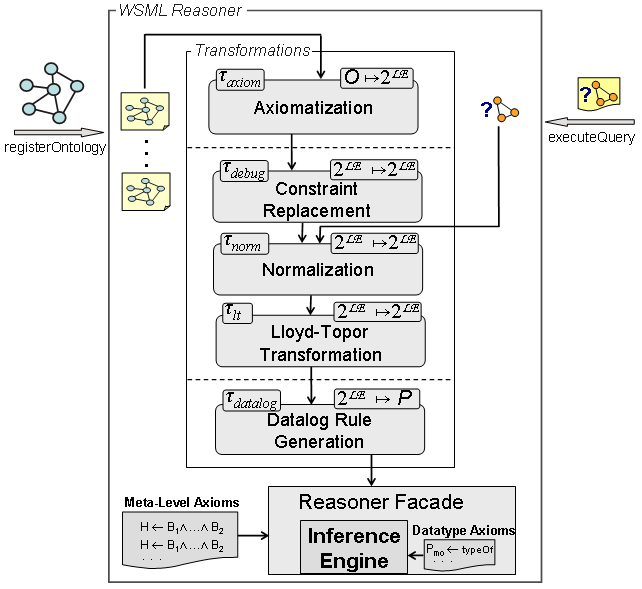
\includegraphics[width=0.76\textwidth]{figures/layering.png}
    \centering
    \caption{Internal framework architecture.
    \label{fig:layering}}\vspace{-5mm}
\end{figure}
Figure~\ref{fig:layering} shows the internal architecture of the
framework as well as the data flow during a prototypical usage
scenario. The outer box outlines a WSML reasoner component that
allows a user to register WSML ontologies and to pose queries on
them. The inner box illustrates the transformation pipeline
introduced in Section \ref{sec:mapping} and shows its subsequent
steps in a layering scheme.

Registered ontologies go through all the transformation steps,
whereas user queries are injected at a later stage, skipping the
non-applicable axiomatization and constraint replacement steps.
Here, the internal layering scheme allows for an easy
reorganization and reuse of the transformation steps on demand,
assuring high flexibility and modularity. A good example for this
is the constraint replacement transformation \transdebug: if
included in the pipeline, it produces the rules that activate the
debugging features according to Section \ref{sec:debugging}; if
excluded, the constraints remain in the resulting Datalog program
and are mapped to native constraints of the underlying reasoning
engine.

The core component of the framework is an exchangeable Datalog
inference engine wrapped by a reasoner facade which embeds it in the
framework infrastructure. This facade mediates between the generic
Datalog program produced in the transformations and the external
engine's tool-specific Datalog implementation and built-in
predicates.\\[2mm]
{\bfseries Interface and Integration with Existing Technology.}
Our framework is based on the WSMO4J
\footnote{\url{http://wsmo4j.sourceforge.net}} project, which
provides an API for the programmatic handling of WSML documents.
WSMO4J performs the task of parsing and validating WSML ontologies
and provides the source object model for our translations. For a
reasoner to be connected to the Framework, a small adapter class
needs to be written, that translates generic Datalog elements to
their equivalent constructs within the internal representation
layer of the underlying reasoner. Our framework currently comes
with facades for two built-in reasoners:
KAON2\footnote{\url{http://kaon2.semanticweb.org}} and
MINS\footnote{\url{http://dev1.deri.at/mins}}. The initial
development was done with the KAON2 inference engine that, with
respect to the challenges for datatype reasoning, provides a very
flexible type system that allows for user-defined datatypes,
together with predicates on these datatypes, including type
checking predicates. However, KAON2 cannot be used for reasoning
in WSML-Rule as it does not support function symbols and unsafe
rules. The second reasoner, MINS, can be used for the WSML-Rule
variant but has limited support for datatype reasoning. (For
determining the WSML variant of an ontology, one can use the
validation facilities built into WSMO4J
%\footnote{A demo of this
%feature is available at:
%\url{http://tools.deri.org/wsml/validator}}
.)
